\documentclass[10pt]{beamer}

\usetheme[progressbar=frametitle, sectionpage=none]{metropolis}
\usepackage{appendixnumberbeamer}

\usepackage{booktabs}
\usepackage[scale=2]{ccicons}

\usepackage{pgfplots}
\usepgfplotslibrary{dateplot}

\usepackage{xspace}
\newcommand{\themename}{\textbf{\textsc{metropolis}}\xspace}

\usepackage[portuguese]{babel}
\usepackage{hyphenat}

\usepackage{courier}

\usepackage{listings}
\usepackage{xcolor}

\usepackage{graphicx}
\usepackage{animate}

\usepackage{tikz}
\usetikzlibrary{graphs}

\lstdefinelanguage{alloy-lang} {
  morekeywords={ abstract, all, var, and, as, assert, but, check, disj, else, exactly, extends, fact, for, fun, iden, iff, implies, in, Int, let, lone, module, no, none, not, one, open, or, pred, run, set, sig, some, sum, univ },
  comment=[l]{--},
  % comment=[s]{/*}{*/}
}

\definecolor{dark-metro}{HTML}{23373b}
\definecolor{light-brown}{HTML}{EB811B}
\definecolor{codegray}{rgb}{0.5,0.5,0.5}

\lstdefinestyle{customstyle}{
    commentstyle=\color{light-brown},
    keywordstyle=\bfseries\color{dark-metro},
    numberstyle=\tiny\color{codegray},  
    basicstyle=\ttfamily\footnotesize,
    breakatwhitespace=false,         
    breaklines=true,                 
    captionpos=b,                    
    keepspaces=true,    
    numbers=left,                    
    numbersep=5pt,                  
    showspaces=false,                
    showstringspaces=false,
    showtabs=false,                  
    tabsize=2,
}

\lstset{style=customstyle}

\renewcommand\lstlistingname{Snippet}

\title{Sea of Thieves em Alloy}
\subtitle{Formulando o universo de Sea of Thieves em Alloy}
\date{\today}
\author{Vinicius S. Gomes}
\institute{Universidade Federal de Minas Gerais}

\begin{document}

\maketitle

\begin{frame}{Sumário}
  \setbeamertemplate{section in toc}[sections numbered]
  \tableofcontents
\end{frame}

\section{O que é Sea of Thieves?}
\begin{frame}[standout]
  O que é Sea of Thieves?
\end{frame}

\begin{frame}[fragile]{O que é Sea of Thieves?}
  \textbf{Sea of Thieves (SoT)} é um jogo \textit{multiplayer} de aventura em mundo aberto, desenvolvido pela Rare e publicado pela Xbox Game Studios.

  É ambientado num universo pirata, no qual jogadores exploram livremente o mapa, enfrentam desafios e interagem entre si em tempo real, seja de forma cooperativa ou competitiva.

  O foco do jogo está em:
  \begin{itemize}
    \item Exploração
    \item Missões colaborativas
    \item Combate terrestre e naval
    \item Interações emergentes entre jogadores e com o mundo
  \end{itemize}
\end{frame}

\begin{frame}[fragile]{Características do jogo}
  \begin{itemize}
    \item Os jogadores assumem o papel de piratas
    \item Possui um vasto mundo para explorar
    \begin{itemize}
      \item Ilhas, ruínas, artefatos misteriosos, etc
    \end{itemize}
    \item A experiência é otimizada para jogar em grupo, seja com amigos ou com outros jogadores online
    \item Além de procurar tesouros, os jogadores podem pescar, caçar, enfrentar capitães esqueletos e participar de batalhas navais
    \item O jogo possui um estilo visual \textit{cartoonizado} e uma física exagerada
  \end{itemize}
\end{frame}

\begin{frame}[fragile]{Gameplay}
  \begin{figure}
    \includegraphics[width=0.8\textwidth]{assets/gameplay-2.jpg}
    \label{fig:gameplay-2}
    \caption{Imagem promocional do jogo.}
    \end{figure}
\end{frame}

\begin{frame}[fragile]{Gameplay}
  \begin{figure}
    \animategraphics[autoplay,loop,width=0.9\textwidth]{24}{assets/gameplay-3/gameplay-3-}{0}{34}
    \label{fig:gameplay-3}
    \caption{Gameplay do jogo.}
  \end{figure}
\end{frame}

\begin{frame}[fragile]{Gameplay}
  \begin{figure}
    \animategraphics[autoplay,loop,width=0.9\textwidth]{24}{assets/gameplay-4/gameplay-4-}{0}{87}
    \label{fig:gameplay-4}
    \caption{Gameplay do jogo.}
  \end{figure}
\end{frame}

% ---

\section{Modelando SoT em Alloy}
\begin{frame}[standout]
  Modelando SoT em Alloy
\end{frame}

\begin{frame}[fragile]{Modelando SoT em Alloy}
  \begin{itemize}
    \item Simplificações realizadas
    \item Assinaturas
    \item Sistema de transição
    \item Propriedades esperadas (\textit{assertions})
    \item Exemplos
  \end{itemize}
\end{frame}

\subsection{Simplificações realizadas}
\begin{frame}[fragile]{Simplificações realizadas}
  \begin{itemize}
    \item a
    \item b
    \item c
    \item d
    \item e
  \end{itemize}
\end{frame}

\begin{frame}[fragile]{Simplificações realizadas}
  \begin{figure}
    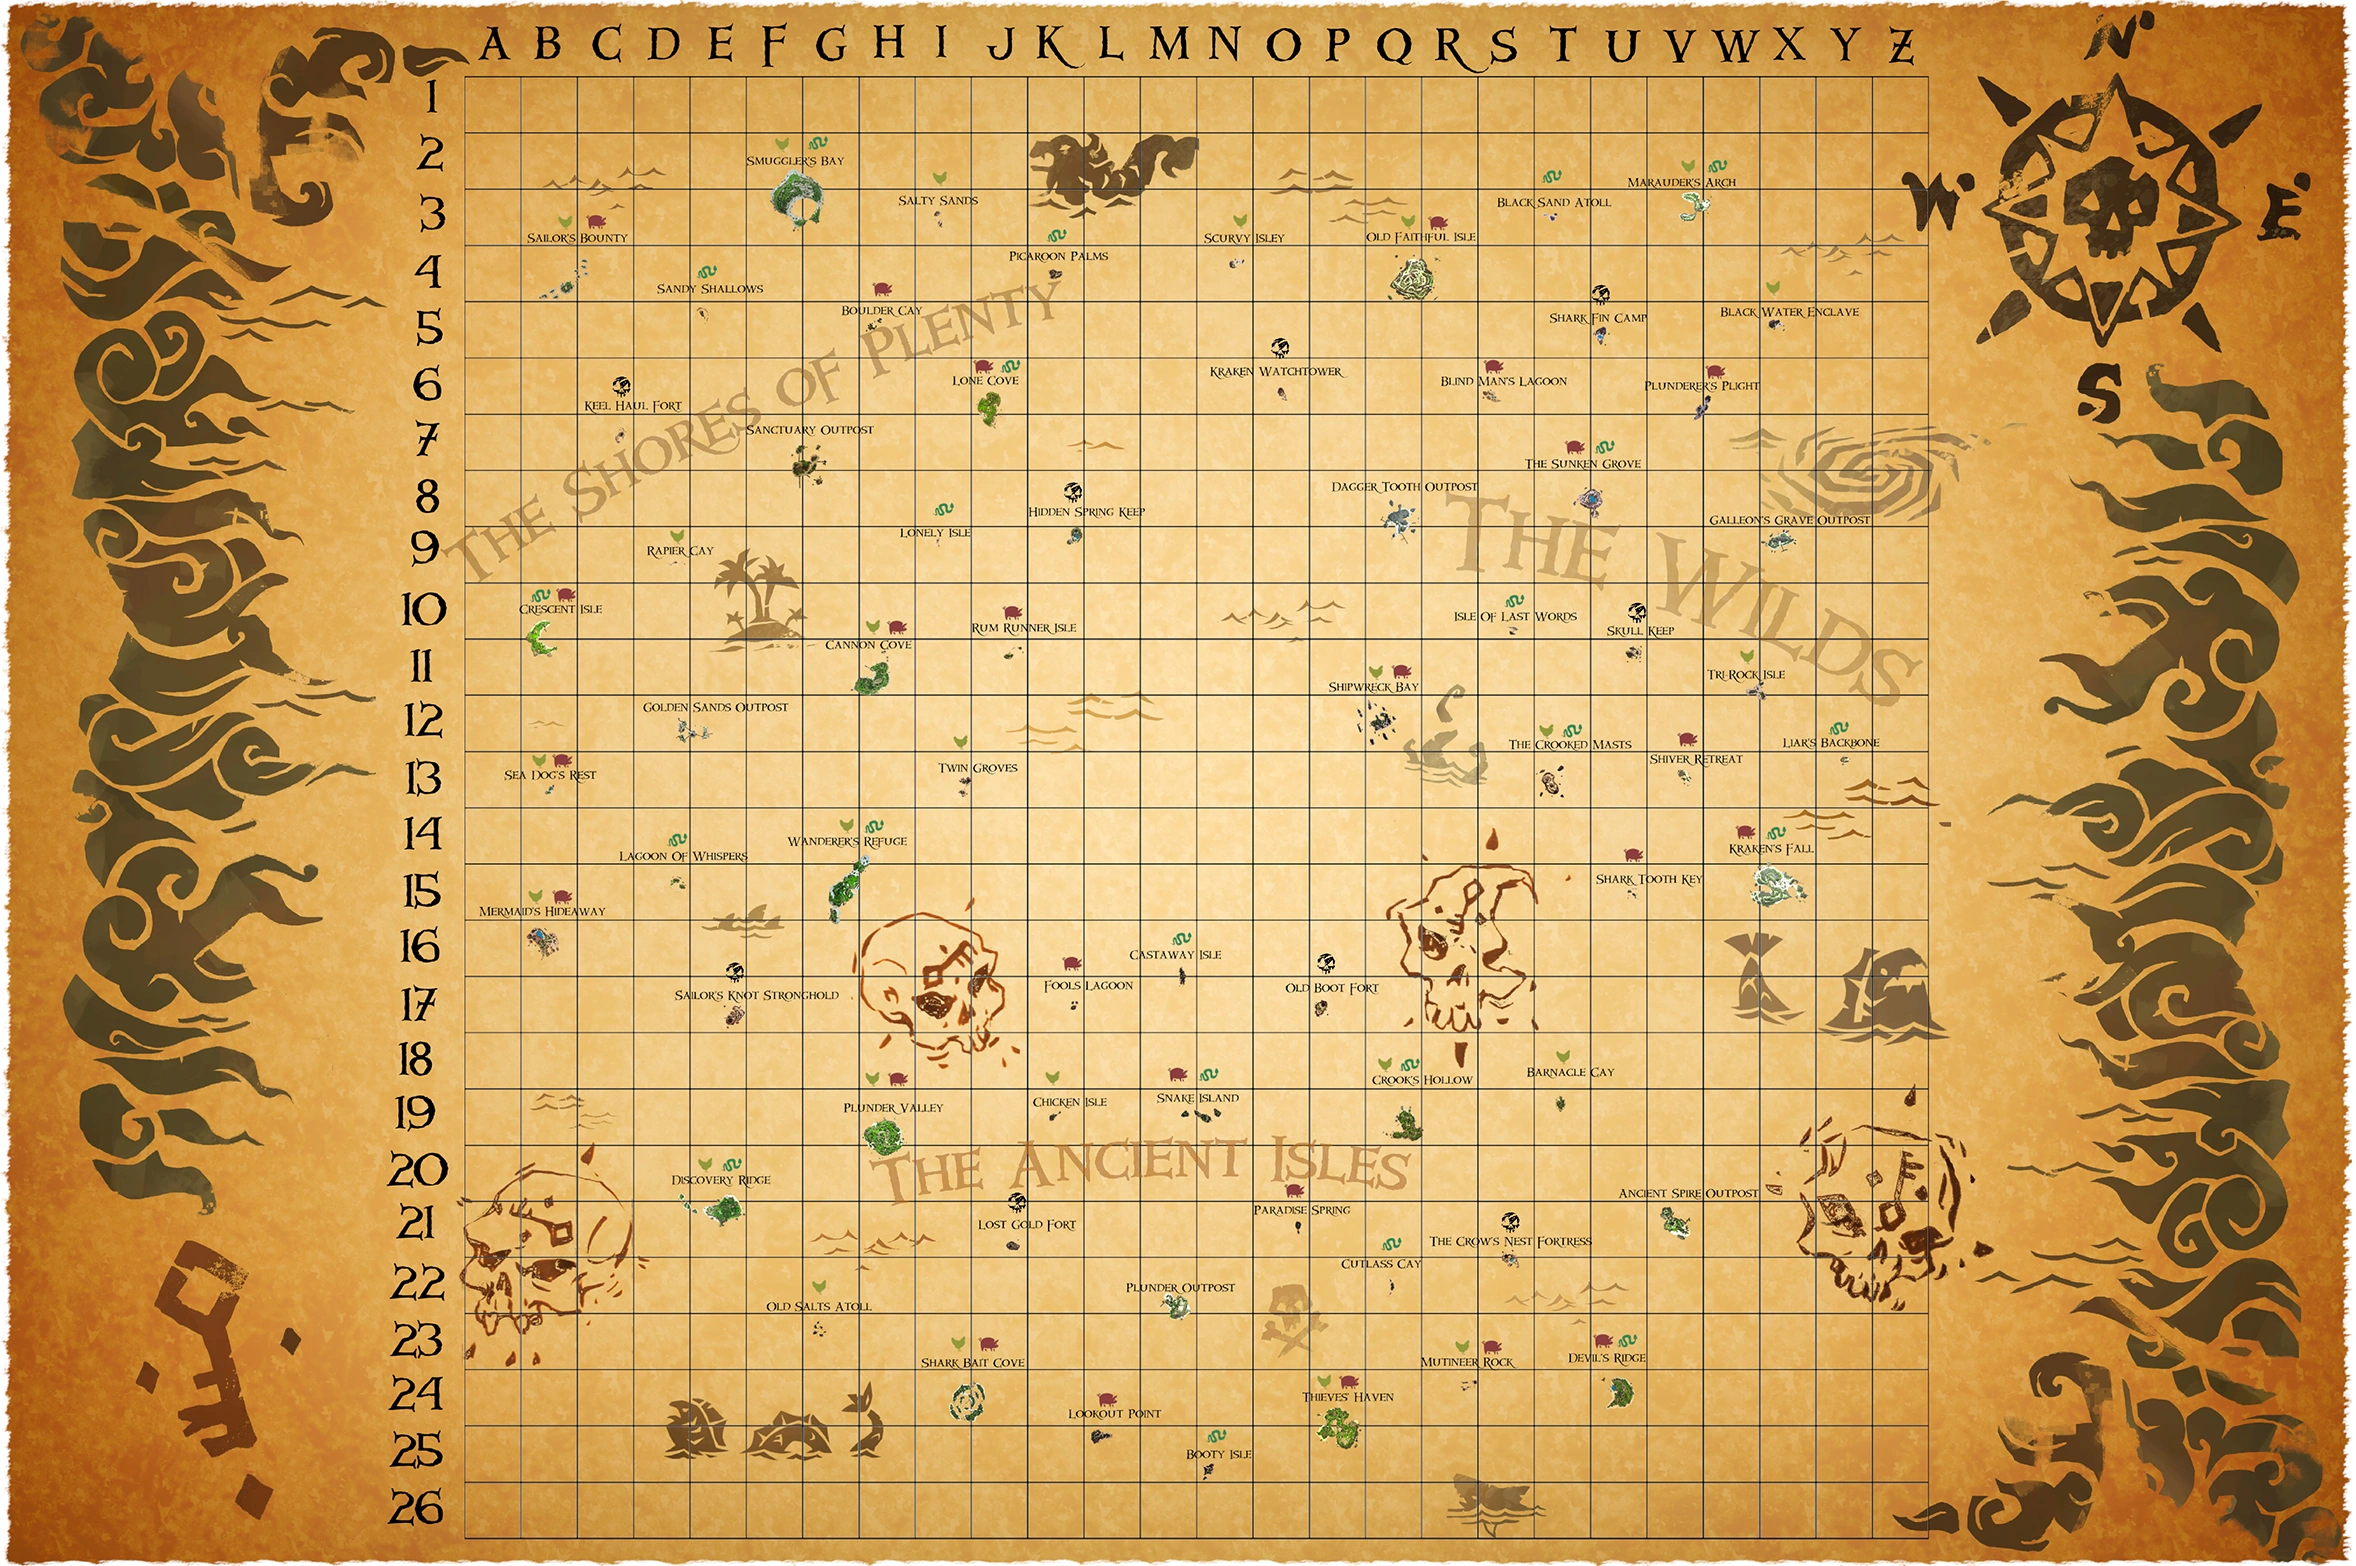
\includegraphics[width=0.9\textwidth]{assets/map.png}
    \label{fig:map}
    \caption{Mapa completo do jogo.}
  \end{figure}
\end{frame}

\begin{frame}[fragile]{Simplificações realizadas}
  \begin{center}
    a
  \end{center}
\end{frame}

\subsection{Assinaturas}
\begin{frame}[fragile]{Assinaturas}
  \begin{lstlisting}[language=alloy-lang, caption=Assinaturas de SoT em Alloy.]
    sig Enemy {}
    sig Treasure {}

    abstract sig Location {}
    one sig Ocean extends Location {}
    sig Island extends Location {
      var treasures: set Treasure,
      var enemies: set Enemy
    }
    sig Outpost extends Location {}

    abstract sig Ship {
      var shipHp: lone Int
    }
    sig Sloop, Brigantine, Galleon extends Ship {}\end{lstlisting}
\end{frame}

\begin{frame}[fragile]{Assinaturas}
  \begin{lstlisting}[language=alloy-lang, caption=Assinaturas de SoT em Alloy.]
    abstract sig PirateStatus {}
    one sig Dead, Alive, Otherworld extends PirateStatus {}

    sig Pirate {
      var hp: lone Int,
      var status: lone PirateStatus
    }

    sig Tripulation {
      var pirates: set Pirate,
      var ship: lone Ship,
      var location: lone Location,
      var collectedTreasures: set Treasure,
      var money: lone Int,
      var resources: lone Int
    }\end{lstlisting}
\end{frame}

\begin{frame}[fragile]{Assinaturas}
  \begin{lstlisting}[language=alloy-lang, caption=Assinaturas de SoT em Alloy.]
    sig Server {
      var tripulations: set Tripulation
    }

    one sig SoTGame {
      servers: set Server
    }

    abstract sig Operator {}
    one sig NOP, ... extends Operator {}
    one sig Track {
      var op: lone Operator
    }\end{lstlisting}
\end{frame}

\subsection{Sistema de transição}
\begin{frame}[fragile]{Sistema de transição}
  d
\end{frame}

\subsection{Propriedades esperadas}
\begin{frame}[fragile]{Propriedades esperadas}
  e
\end{frame}

\subsection{Exemplos}
\begin{frame}[fragile]{Exemplos}
  f
\end{frame}

% ---

\section{Considerações finais}
\begin{frame}[standout]
  Considerações finais
\end{frame}

\begin{frame}[fragile]{Considerações finais}
  \begin{itemize}
    \item a
    \item b
    \item c
  \end{itemize}
\end{frame}

\appendix

% \begin{frame}[allowframebreaks]{Referências}
%   \bibliography{bibliography}
%   \bibliographystyle{abbrv}
% \end{frame}

\begin{frame}[standout]
  Perguntas?
\end{frame}

\end{document}
